\documentclass{article}
\usepackage[a4paper, margin=2.5cm, headheight=13pt]{geometry}
\usepackage[T1]{fontenc}
\usepackage[french]{babel}
\usepackage{fancyhdr}
\usepackage{xurl}

% Figures
\usepackage{tikz}
\usetikzlibrary{positioning, calc}
\usepackage{graphicx}
\usepackage{caption}
\usepackage{subcaption}

% Références
\usepackage{csquotes}
\usepackage{biblatex}
\addbibresource{ref.bib}

%define_color
\definecolor{bleu}{rgb}{0,0.52,1}
\definecolor{vert}{rgb}{0.45,0.82,0}
\definecolor{violet}{rgb}{0.51,0.13,0.55}

% Définir la pagination etc.
\pagestyle{fancy}
\fancyhf{}
\lhead{MICRO-315 Miniprojet} 
\rhead{Les aventures de Jean-Bot}
\fancyfoot
{
    \begin{tikzpicture}[remember picture,overlay]
            \node[] (chat) at ($(current page.south)+(0,1.5)$) {
\includegraphics[width=1cm]{images/amour.pdf}};
            \node[] () at ($(chat)+(0,0.04)$) {\thepage};
            \node[] () at ($(chat)-(1,0)$) {
\includegraphics[width=1cm]{images/kawwai.pdf}};
            \node[] () at ($(chat)+(1,0)$) {\scalebox{-1}[1]{
\includegraphics[width=1cm]{images/kawwai.pdf}}};
    \end{tikzpicture}
}

\newcommand{\state}{\colorbox{yellow}{\textbf{ManagesStates}}}
\newcommand{\dance}{\colorbox{yellow}{\textbf{Dance}}}

\begin{document}
    \begin{titlepage}
        \begin{tikzpicture}[remember picture, overlay]
            \node[] () at (current page.center) {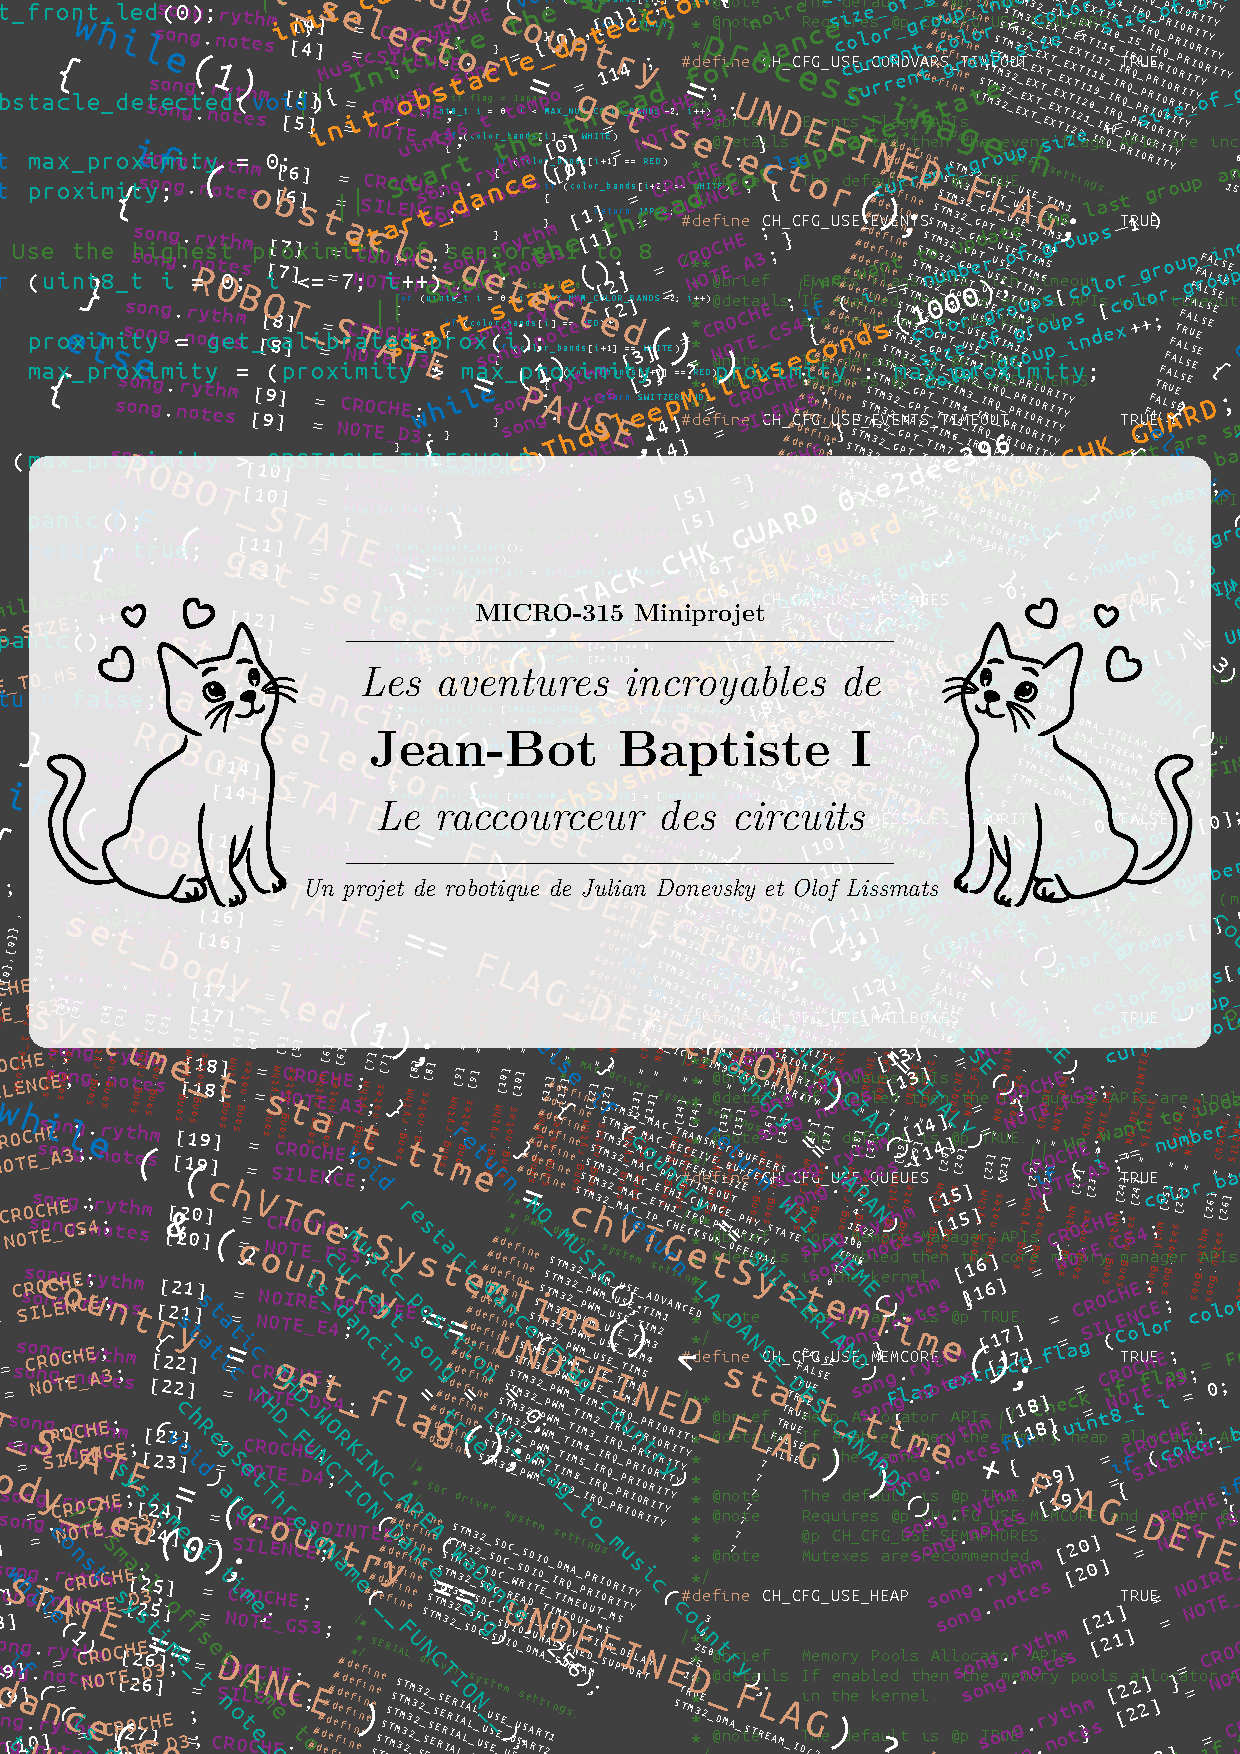
\includegraphics[width=\paperwidth]{couverture/couverture.pdf}};
        \end{tikzpicture}
        
        \vspace*{\fill}
        
        \begin{center}
            \begin{tikzpicture}[remember picture, overlay]
                \fill[color = white, opacity = 0.85, rounded corners = 2ex] (-10,5) rectangle (10,-5);
                \node (titre) at (0,0)
                    {
                        \begin{tabular}{c}
                            \hline
                            \\
                            \huge\it Les aventures incroyables de \\
                            \\
                            \Huge\bf Jean-Bot I$^\textbf{\Large er}$ \\
                            \\
                            \huge\it Le raccourceur de circuits\\
                            \\
                            \hline
                        \end{tabular}
                    };
                \node[above] at (titre.north) {\textbf{\large MICRO-315 Miniprojet}};
                \node[below] at (titre.south) {\textit{\large Un projet de robotique de Julian Donevsky et Olof Lissmats}};
            \end{tikzpicture}
        \end{center}
        
        \vspace{5cm}
        
        \vspace*{\fill}
    \end{titlepage}

    \thispagestyle{empty}

    \tableofcontents
    
    \vfill
    
    \noindent Illustration de couverture : Julian Donevsky et Olof Lissmats
    
    \noindent Chat de décoration : NicePNG, Better Cats Drawing Pictures Wealth How To Draw A Cute - Cat Drawing, téléchargé le 12 mai 2022, <\url{https://www.nicepng.com/ourpic/u2w7a9a9i1y3q8t4_better-cats-drawing -pictures-wealth-how-to-draw/}>

    \newpage

    \setcounter{page}{1}

    \section{Introduction}

    Dans le cadre de ce projet, nous avons créé un programme qui permet au robot de danser sur une musique en particulier en fonction d'un drapeau de pays que l'utilisateur lui présente.
    Le robot utilise ses capteurs de proximités infrarouges pour s'assurer qu'aucun obstacle ne bloque son chemin lorsqu'il danse. 
    Si c'est le cas, il arrête temporairement sa danse jusqu'à ce que l'obstacle soit dégagé.

    \section{Fonctionnement du programme}
    
    \subsection{Schéma général du programme}
    \begin{figure}[!ht]
        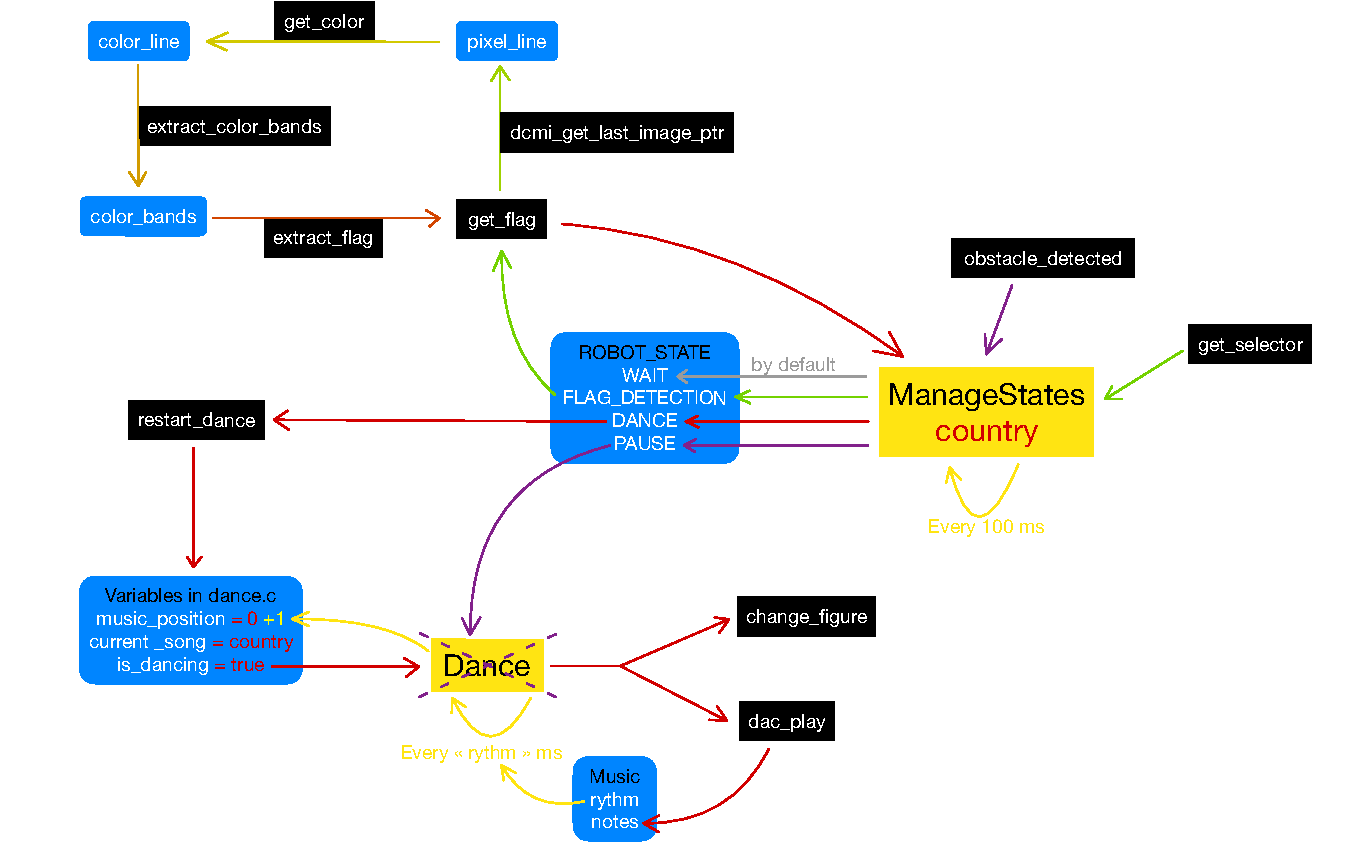
\includegraphics[scale=0.7]{images/code-structure.pdf}
        \caption{Schéma général du programme. En jaune les threads, en noir les fonctions et en bleu (rouge dans le cas de country) les variables utiles au bon déroulement du programme.}
        \label{fig:structure} % Pour référer à cette figure dans le texte
    \end{figure}

    L'utilisateur tourne le selecteur (peu importe de combien de cran). 
    La détection se fait en appellant la fonction \textbf{get$\_$selector} dans le thread \colorbox{yellow}{\textbf{ManagesStates}}, qui met ensuite l'état du robot à \textcolor{bleu}{FLAG$\_$DETECTION} ce qui a pour conséquence d'appeler la fonction \textbf{get$\_$flag} (\textcolor{vert}{flèche en vert}). \\ \par
    
    La fonction \textbf{get$\_$flag} analyse la dernière image capturée par la caméra puis en déduit le drapeau présenté, de la manière décrite dans la section \ref{get_flag}.
    Au cas où le drapeau détecté n'est pas défini, elle continue de s'exécuter en boucle jusqu'à obtenir un drapeau connu pendant au maximum 10 secondes. 
    Passé ce délai, le robot retourne dans l'état \textcolor{bleu}{WAIT}. \\ \par
    
    Lorsqu'un drapeau connu est trouvé, le thread \colorbox{yellow}{\textbf{ManagesStates}} appelle la fonction \textbf{restart$\_$dance} qui réveille le thread \colorbox{yellow}{\textbf{Dance}} (\textcolor{red}{flèche en rouge}). 
    En effet, la variable \textcolor{bleu}{is$\_$dancing} est initialisée à \textit{false} et inhibe le thread en le faisant simplement dormir dans une boucle de 100 ms. 
    Lorsqu'elle passe à \textit{true}, celui-ci sort de son sommeil et commence à jouer la musique \textcolor{bleu}{current$\_$song}.
    Cette dernière est changée à la musique du pays détecté par \textbf{restart$\_$dance} grâce à une look up table. 
    A chaque note jouée, les fonctions \textbf{change$\_$figure} et \textbf{dac$\_$play} sont appelée pour changer de mouvement de dance en activant de façon aléatoire les moteurs et jouer le son voulu, respectivement. 
    De plus, la variable \textcolor{bleu}{music$\_$position} indiquant quelle note et rythme jouer de la structure \textcolor{bleu}{Music} est incrémentée. \\ \par
    
    A chaque appel de \state, \textbf{obstacle\_detected} est appelé pour vérifier qu'aucun obstacle n'obstrue le chemin du robot lorsqu'il danse. 
    Si tel est le cas, le robot passe en mode \textcolor{bleu}{PAUSE}, ce qui a pour conséquence d'inhiber le thread \dance en le faisant retourner dans sa boucle de sommeil de 100 ms (\textcolor{violet}{flèche en violet}). 
    Une fois l'obstacle enlevé, le robot continue sa danse en reprenant là où il s'était arrêté. 
    À noter que la détection d'obstacle n'affecte nullement la détection de drapeau car les fonctions gérants ces deux tâches sont appelées depuis le même thread, soit \state.
    Elles se bloquent donc mutuellement.
    Ceci est complètement maîtrisé.
    Lorsque le robot est en train de détecter le drapeau, il ne doit faire que cela.

    \subsection{La fonction get\_flag}
    \label{get_flag}
    
    \begin{figure}[!ht]
        \noindent\makebox[\textwidth]{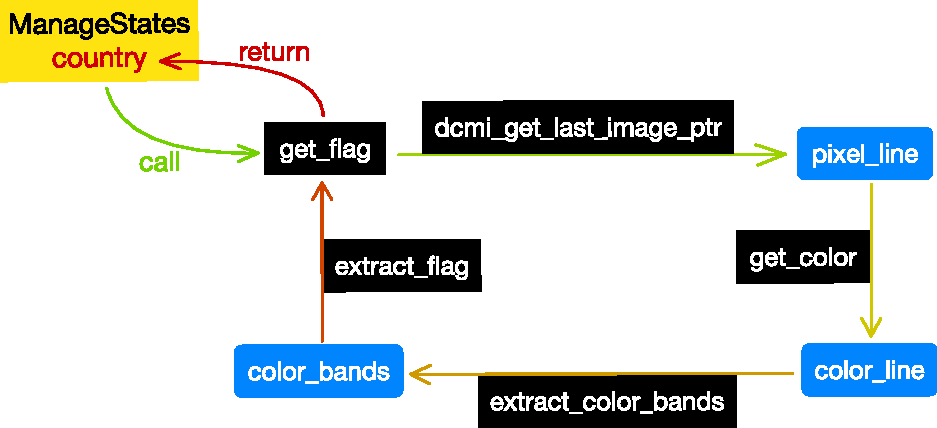
\includegraphics[scale=0.6]{docs/rapport/images/get_flag.pdf}}
        \caption{Schéma de la fonction \textbf{get\_flag}.}
        \label{fig:get_flag} % Pour référer à cette figure dans le texte
    \end{figure}
    
    A chaque appel de \textbf{get\_flag}, une ligne horizontale de la dernière image capturée par la caméra est stockée dans la variable \textcolor{bleu}{pixel\_line}. 
    La fonction \textbf{get\_color} convertit chaque pixel de cette dernière variable en une couleur: \textit{WHITE, RED, GREEN, BLUE, UNDEFINED\_COLOR}, puis les stocke dans \textcolor{bleu}{color\_line}, un array de type \textit{Color}. 
    Le fonctionnement de \textbf{get\_color} est décrit plus en détail dans la section \ref{améliorer_couleur}. 
    La fonction \textbf{extract\_color\_bands} décrite dans la section \ref{extract_color_bands} analyse ce vecteur en extrayant les bandes de couleurs correspondant au drapeau puis les stocke dans \textcolor{bleu}{color\_bands}. 
    Finalement, \textbf{extract\_flag} analyse ces bandes et en déduit le drapeau correspondant.
    
    \subsection{La fonction extract\_color\_bands}
    \label{extract_color_bands}
    \begin{figure}[!ht] %{\textwidth}
        \begin{center}
            \begin{tikzpicture}[scale=0.3]
                \foreach \i in {1,...,4}
                {
                    \draw[fill=gray] (\i,0) rectangle (\i+1,2);
                }
                \foreach \i in {5,...,8}
                {
                    \draw[fill=red] (\i,0) rectangle (\i+1,2);
                }
                \foreach \i in {9,...,11}
                {
                    \draw[fill=green] (\i,0) rectangle (\i+1,2);
                }
                \foreach \i in {12,...,13}
                {
                    \draw (\i,0) rectangle (\i+1,2);
                }
                \foreach \i in {14,...,23}
                {
                    \draw[fill=blue] (\i,0) rectangle (\i+1,2);
                }
                \foreach \i in {24,...,27}
                {
                    \draw (\i,0) rectangle (\i+1,2);
                }
                \draw[fill=green] (28,0) rectangle (29,2);
                \foreach \i in {29,...,34}
                {
                    \draw (\i,0) rectangle (\i+1,2);
                }
                \foreach \i in {35,...,44}
                {
                    \draw[fill=red] (\i,0) rectangle (\i+1,2);
                }
            \end{tikzpicture}
        \end{center}
        \caption{Une fois les valeurs RGB de chaque pixel converties en couleurs, elles sont stockées de cette manière. La couleur grise représente ici \textit{UNDEFINED$\_$COLOR}. Voici un exemple de \textcolor{bleu}{color$\_$line} simplifié avec seulement avec 44 pixels (contre 640 en réalité). Le drapeau français est ici présenté à la caméra (légèrement décalé à droite) avec une erreur de couleur dans la bande blanche et à gauche un peu de bruit lié à l'environnement derrière le drapeau.}
    \end{figure}

    \vspace{5mm}

    \begin{figure}[!ht] %{\textwidth}
        \begin{center}
            \begin{tikzpicture}[scale=0.4]
                \draw[fill=gray]  (0,3) rectangle (1,5) node[midway] (A) {};
                \draw[fill=red]   (1,3) rectangle (2,5);
                \draw[fill=green] (2,3) rectangle (3,5);
                \draw[fill=white] (3,3) rectangle (4,5);
                \draw[fill=blue]  (4,3) rectangle (5,5);
                \draw[fill=white] (5,3) rectangle (6,5);
                \draw[fill=green] (6,3) rectangle (7,5);
                \draw[fill=white] (7,3) rectangle (8,5);
                \draw[fill=red]   (8,3) rectangle (9,5);
                \node[anchor=east] () at ($(A)-(1,0)$) {\texttt{color\_groups:}};

                \draw (0,0) rectangle (1,2) node[midway] (B) {\texttt{4}};
                \draw (1,0) rectangle (2,2) node[midway] {\texttt{4}};
                \draw (2,0) rectangle (3,2) node[midway] {\texttt{3}};
                \draw (3,0) rectangle (4,2) node[midway] {\texttt{2}};
                \draw (4,0) rectangle (5,2) node[midway] {\texttt{10}};
                \draw (5,0) rectangle (6,2) node[midway] {\texttt{4}};
                \draw (6,0) rectangle (7,2) node[midway] {\texttt{1}};
                \draw (7,0) rectangle (8,2) node[midway] {\texttt{6}};
                \draw (8,0) rectangle (9,2) node[midway] {\texttt{10}};
                \node[anchor=east] () at ($(B)-(1,0)$) {\texttt{size\_of\_groups:}};
            \end{tikzpicture}
        \end{center}
        \caption{Les pixels sont d'abord groupés en fonction de leurs couleurs dans deux arrays \texttt{color\_groups} et \texttt{size\_of\_groups} qui contiennent la couleur et la taille du groupe respectivement.}
    \end{figure}

    \vspace{5mm}

    \begin{figure}[!ht] %{\textwidth}
        \begin{center}
            \begin{tikzpicture}[scale=0.4]
                \draw[fill=gray]  (0,3) rectangle (1,5) node[midway] (A) {};
                \draw[fill=red]   (1,3) rectangle (2,5);
                \draw[fill=blue]  (2,3) rectangle (3,5);
                \draw[fill=white] (3,3) rectangle (4,5);
                \draw[fill=white] (4,3) rectangle (5,5);
                \draw[fill=red]   (5,3) rectangle (6,5);
                \node[anchor=east] () at ($(A)-(1,0)$) {\texttt{color\_groups:}};

                \draw (0,0) rectangle (1,2) node[midway] (B) {\texttt{4}};
                \draw (1,0) rectangle (2,2) node[midway] {\texttt{4}};
                \draw (2,0) rectangle (3,2) node[midway] {\texttt{10}};
                \draw (3,0) rectangle (4,2) node[midway] {\texttt{4}};
                \draw (4,0) rectangle (5,2) node[midway] {\texttt{6}};
                \draw (5,0) rectangle (6,2) node[midway] {\texttt{10}};
                \node[anchor=east] () at ($(B)-(1,0)$) {\texttt{size\_of\_groups:}};
            \end{tikzpicture}
        \end{center}

        \caption{Un premier nettoyage est effectué pour éliminer le bruit et éventuelles erreurs de couleurs en supprimant tous les petits groupes de couleurs (moins de 4 pixels dans l'exemple simplifié).}
    \end{figure}

    \vspace{5mm}

    \begin{figure}[!ht] %{\textwidth}
        \begin{center}
            \begin{tikzpicture}[scale=0.4]
                \draw[fill=gray]  (0,3) rectangle (1,5) node[midway] (A) {};
                \draw[fill=red]   (1,3) rectangle (2,5);
                \draw[fill=blue]  (2,3) rectangle (3,5);
                \draw[fill=white] (3,3) rectangle (4,5);
                \draw[fill=red]   (4,3) rectangle (5,5);
                \node[anchor=east] () at ($(A)-(1,0)$) {\texttt{color\_groups:}};

                \draw (0,0) rectangle (1,2) node[midway] (B) {\texttt{4}};
                \draw (1,0) rectangle (2,2) node[midway] {\texttt{4}};
                \draw (2,0) rectangle (3,2) node[midway] {\texttt{10}};
                \draw (3,0) rectangle (4,2) node[midway] {\texttt{10}};
                \draw (4,0) rectangle (5,2) node[midway] {\texttt{10}};
                \node[anchor=east] () at ($(B)-(1,0)$) {\texttt{size\_of\_groups:}};
            \end{tikzpicture}
        \end{center}

        \caption{Les groupes de mêmes couleurs consécutives sont fusionnés.}
    \end{figure}

    \vspace{5mm}
    
    \begin{figure}[!ht] %{\textwidth}
        \begin{center}
            \begin{tikzpicture}[scale=0.4]
                \draw[fill=gray]  (0,3) rectangle (1,5) node[midway] (A) {};
                \draw[fill=gray]   (1,3) rectangle (2,5);
                \draw[fill=blue]  (2,3) rectangle (3,5);
                \draw[fill=white] (3,3) rectangle (4,5);
                \draw[fill=red]   (4,3) rectangle (5,5);
                \node[anchor=east] () at ($(A)-(1,0)$) {\texttt{color\_groups:}};

                \draw (0,0) rectangle (1,2) node[midway] (B) {\texttt{4}};
                \draw (1,0) rectangle (2,2) node[midway] {\texttt{4}};
                \draw (2,0) rectangle (3,2) node[midway] {\texttt{10}};
                \draw (3,0) rectangle (4,2) node[midway] {\texttt{10}};
                \draw (4,0) rectangle (5,2) node[midway] {\texttt{10}};
                \node[anchor=east] () at ($(B)-(1,0)$) {\texttt{size\_of\_groups:}};
            \end{tikzpicture}
        \end{center}

        \caption{Un second nettoyage est effectué pour supprimer les groupes qui sont trop petits pour être considérés comme des bandes d'un drapeau. Dans le programme, ils sont simplement changé à \textit{UNDEFINED$\_$COLOR}.}
    \end{figure}

    \vspace{5mm}

    \begin{figure}[!ht] %{\textwidth}
        \begin{center}
            \begin{tikzpicture}[scale=0.4]
                \draw[fill=gray]  (0,3) rectangle (1,5) node[midway] (A) {};
                \draw[fill=blue]  (1,3) rectangle (2,5);
                \draw[fill=white] (2,3) rectangle (3,5);
                \draw[fill=red]   (3,3) rectangle (4,5);
                \node[anchor=east] () at ($(A)-(1,0)$) {\texttt{color\_groups:}};
            \end{tikzpicture}
        \end{center}

        \caption{Finalement, les \textit{UNDEFINED$\_$COLOR} consécutifs sont à nouveau fusionné en s'affranchissant cette fois de \texttt{size\_of\_groups}. Le vecteur de couleur de cette dernière étape est retourné en tant que \textcolor{bleu}{color$\_$bands} pour être ensuite analysé par la fonction \textbf{extract$\_$flag}.}
    \end{figure}

    \section{Problèmes apparus lors du projet}
    
    \subsection{Détecter la bonne couleur de pixel}
    \label{problème_couleurs}
    Lors des premiers tests que nous avons effectués avec la caméra, nous utilisions des drapeaux imprimés sur papier. 
    A cause des reflets et du changement de luminosité, il était quasiment impossible de paramétrer la détection de couleur pour qu'elle fonctionne à tous les coups, c'est pourquoi nous utilisons maintenant un écran comme support pour les drapeaux.
    
    \subsection{Détacher les notes de musiques qui se répètent}
    Lors des premiers tests musicaux, nous avons remarqué que le robot ne détachait pas 2 notes identiques consécutives. Nous avons dû donc modifier le thread \colorbox{yellow}{\textbf{Dance}} pour qu'il arrête de jouer une note quelques millisecondes avant de jouer la suivante sans toutefois s'arrêter de danser. Cependant, un problème subsistait: lorsque la musique était finie ou bien lorsqu'une note très rapide devait être jouée, le programme plantait. En effet, le robot devait s'arrêter de jouer la note avant même de l'avoir commencée. Nous avons dû donc ajouter une condition à ce détachement de note, qui fonctionne maintenant très bien sans poser de problème.
    
    \subsection{Optimiser l'accès en mémoire des musiques}
    Initialement, lorsque nous avions besoin d'accéder à un morceau pour le stocker dans la variable \textcolor{bleu}{current\_song} à l'appel de \textbf{restart\_dance}, nous faisions appel à une fonction qui calcule chaque composante du morceau puis le recopie dans \textcolor{bleu}{current\_song}. 
    Ce n'était pas optimal car lorsque l'on présente plusieurs fois le même drapeau, le robot va recalculer le même morceau à chaque fois, ce qui est une grosse perte de temps. 
    De façon similaire à la fonction sinus, nous avons ainsi créé une fonction \textbf{init\_songs} qui initialise chaque musique au début du programme et les stocke dans des variables de types \textit{Music}, comme expliqué lors du cours 4. \cite{sinus}
   
    \section{Points à améliorer}
    Il y a plusieurs points à améliorer afin d'optimiser notre programme si nous avions eu plus de temps.

    \subsection{Créer un thread propre pour la détection d'obstacles}
    Dans l'état actuel des choses le robot vérifie l'absence d'obstacles en appellant la  fonction au début du thread \colorbox{yellow}{\textbf{ManagesStates}}.
    Par conséquent, un obstacle peut se présenter après cet appel, lorsque le robot est occupé par d'autres tâches, sans causer un arrêt d'activité.
    Cela se produit par exemple pendant la détection des drapeaux où le robot est bloqué dans une boucle.

    L'ajout d'un thread complètement dédié à la détection d'obstacle permettrait d'y réagir à chaque instant, ce qui pourrait être utile.
    En revanche cela impliquerait aussi une nécessité de faire communiquer cette thread avec les autres, c'est à dire introduire plus de variables globales.
    Un autre problème est qu'un nombre plus important de threads nécessiterait un ordonnancement plus complexe par le système d'exploitation, ce qui rend plus difficile de garantir que tous les threads ont suffisamment de temps pour son exécution.
    De plus cela rendrait l'exécution plus lent à cause d'un nombre plus élevé de changement de thread.
    À cause de la taille faible de ce projet, les deux derniers problèmes mentionnés ne serait pas encombrants.
    
    Cette proposition n'est pas une amélioration dans la vraie sens, mais plutôt une variation.
    Elle éviterait un probléme, mais en engendrerait d'autres.
    Comme on considère les problèmes alternatifs plus grands que ceux présents, on a choisi de ne pas implémenter l'alternative.

    \subsection{Rendre la détection de couleurs plus fiable}
    \label{améliorer_couleur}
    La caméra du robot fournit une image de 640 fois 480 pixels sous le format RGB565.
    Cela signifie que l'intensité de rouge, vert et bleu sont représentés sur 5, 6 et 5 pixels respectivement.
    Afin de déterminer la couleur représentée, les écarts entre ces trois valeurs sont analysées par la fonction \textbf{get\_color}.
    Par exemple, si R est plus grand que G et B d'une certaine valeur, le robot en déduit que le pixel est de couleur rouge.
    La détection du vert et du bleu se fait de façon similaire.
    Si les 3 couleurs sont présentes sur le pixel, le robot en déduit qu'il est blanc.
    % Sous supposition que les valeurs RGB sont représentées sur la même échelle, c'est à dire le même nombre de bits, le pourcentage dont une valeur dépasse les autres pourrait être analysé par exemple. 
    
    Comme expliqué dans la section \ref{problème_couleurs}, cette méthode fonctionne très bien avec un écran mais elle fonctionne très mal avec d'autres supports tel que le papier. Nous pourrions améliorer cela en ajoutant d'autres conditions plus précises pour la détection d'une couleur.
    
    \subsection{Optimiser l'utilisation de mémoire des pièces de musique}
    Tous les morceaux de notre robot sont stockés dans une structure de taille fixe appelée \texttt{Music} mesurant $55 \cdot 4 = 220$ bytes. 
    Si nous avions décidé de créer un morceau beaucoup plus long que les autres, nous aurions été obligés d'augmenter la taille en mémoire de cette structure, et ainsi de tous les autres morceaux aussi, ce qui n'est pas optimal. 
    Une manière de corriger le problème aurait été de faire de l'allocation dynamique de mémoire plutôt que d'utiliser une structure fixe. 
    Malheureusement, ceci est assez difficile en C. 
    Nous aurions aussi pu utiliser des pointeurs mais ils peuvent créer des fuites de mémoires s'ils ne sont pas correctement gérés. 
    Nous avons opté sur l'utilisation d'arrays, une solution plus simple mais moins efficace.
    
    
    
    
    \subsection{Autres points mineurs}
    Le robot a certains comportements qui pourraient être codés différemment.
    Il ne s'agit pas de rectifier des problèmes, mais de faire un choix de préférence.
    En voici un liste non-exhaustive ci-dessous : 
    \begin{enumerate}
        \item Les LEDs qui indique qu'un obstacle bloque le chemin pourraient aussi indiquer où est l'obstacle.
        Par exemple le robot pourrait allumer le LED de devant si l'obstacle se situe en face de lui.
        \item Le robot pourrait danser une danse prédéfinie pour chaque pièce de musique au lieu d'en danser une pseudo-aléatoire.
        \item Améliorer la variété des drapeau détectables, par exemple en ajoutant plus de couleurs possible ou bien permettre de détecter les tricolores verticales au lieu de ne détecter que les tricolores horizontales, ce qui est le cas au moment de la rédaction.
        \item Plus de pays pourraient être ajoutés si la mémoire le permet.
    \end{enumerate}
    
    \printbibliography
\end{document}
